
% \documentclass[twoside]{../style/ucasthesis}

\documentclass[oneside]{./style/ucasthesis}
\usepackage[super,list]{./style/artratex}
\usepackage{./style/artracom}

\usepackage{multirow}
\usepackage{longtable}
\usepackage{graphicx}


% \usepackage{algorithm}  
% \usepackage{algpseudocode}  
% \usepackage{amsmath}  
% \renewcommand{\algorithmicrequire}{\textbf{Input:}}  % Use Input in the format of Algorithm  
% \renewcommand{\algorithmicensure}{\textbf{Output:}} % Use Output in the format of Algorithm  



% \lstset{
%     numbers=left,   %添加代码的编号,在左侧
%     basicsytle=\ttfamily,  % //字母使用打字机字族
%     language=C++  %//高亮C++代码
% }

\begin{document}




% \linespread{1.2}
% \tableofcontents



\mainmatter

% \input{../content/base.tex}
% \input{../content/a3.tex}

% \input{../content/planning}

% \input{../content/520plan_interface}
% \section{AMCL}


\subsection{里程计噪声}


% \section{AMCL中odometry的数据处理}



\begin{frame}{AMCL中odom部分参数配置}
  AMCL关于odom的参数配置列表(以差速模型为例):

  % \frametitle{表格}
  \begin{table}[htbp!]
    \centering
    % \caption{}
    \begin{tabular}{c|c|c}
      \toprule[1pt]
      参数	& 默认值 & 描述  \\
      \toprule[1pt]
      odom\_model\_type	& diff & 里程计运动模型,种类有diff、ommi等 \\
 	    \hline
      odom\_alpha1	&  0.2 & 机器人旋转分量中的旋转噪声 \\
      \hline
      odom\_alpha2	&  0.2 & 机器人平移分量中的旋转噪声 \\
      \hline
      odom\_alpha3	&  0.2 & 机器人平移分量中的平移噪声 \\
      \hline
      odom\_alpha4	&  0.2 & 机器人旋转分量中的平移噪声 \\
 	    \bottomrule[1pt]
    \end{tabular}
  \end{table}
\end{frame}

% \begin{frame}
%   \frametitle{里程计运动模型(一)}
%   \begin{itemize}
%     \item 在计算时间$\Delta t$内,控制$u_t = (\nu, \omega)$ 作用下将机器人位姿从$x_{t-1} = (x, y, z)^T$ 
%           变成位姿$x_t = (x^\prime, y^\prime, \theta^\prime)^T$ 的概率$p(x_t | u_t, x_{t-1})$ 。
%     \item 为了保持状态空间比较小,通常把里程计数据认为是控制信号。
%     \item 总之,用距离测量代替控制, 距离是通过里程计编码信息得到的。
%   \end{itemize}

% \end{frame}


  \begin{frame}{里程计运动模型}
    
    \begin{columns}%0.6 0.4表示相对比例
    \column{0.5\textwidth}%<1->
    % \frametitle{条目}
    \begin{itemize}
    \item 里程计差分模型:两平行轮作驱动,另外附加一个万向轮作支撑。
    \item 在AMCL算法中将机器人的每一步的广义运动进行了拆解,拆解成包含三个动作的序列:
      \begin{itemize}
        \item 在起始点旋转,转向终止点的方向
         \item 朝着该方向做直线运动到终止点
         \item 在终止点进行旋转,转到目标方向
      \end{itemize}

    \end{itemize}

    \column{0.5\textwidth}%<1->
    % 分栏的右侧插入了图片。
     \begin{figure}[!h]
      \centering
      % Requires \usepackage{graphicx}
      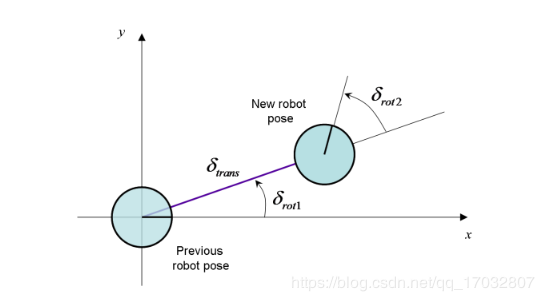
\includegraphics[width=5cm,trim=50 25 50 50,clip]{amcl/odom_model}\\
      % \caption{logo图片样例}\label{pic6}
    \end{figure}
    \begin{itemize}
      \item $\delta_{rot1}$代表在起始点的旋转
      \item $\delta_{trans}$代表着第二段平移过程
      \item $\delta_{rot2}$代表着在终止点的旋转
    \end{itemize}
    \end{columns}
    % 分栏后面的一些内容!!
    \end{frame}

\begin{frame}{里程计运动模型的噪声}
  % \begin{itemize}
	% 	\item 在起始点旋转,转向终止点的方向
	%  	\item 着该方向做直线运动到终止点
	%  	\item 在终止点进行旋转,转到目标方向
  %  \end{itemize}
  \begin{itemize}
  \item 里程计无噪声情况: 里程计读轮子的转圈和机器人的位移是精确对应的。
  \item   理论和仿真可以做到,假设:
    \begin{itemize}
      \item 轮子与地面不打滑
      \item 地面绝对平整
      \item 轮子不变形
      \item 里程计和机器人轮轴之间没有迟滞可以做到完全时间同步,等等
    \end{itemize}
  \item 在AMCL中,里程计是作为{\color{red}状态预测器}存在的,根据控制信息和上一时刻机器人的状态,同时考虑里程计噪声信息,对当前时刻状态进行预测。
  \end{itemize}
\end{frame}  

\begin{frame}
  \frametitle{概率分布采样}

  {\color{red}Box-Muller变换}是通过服从均匀分布的随机变量,来构建服从高斯分布的随机变量的一种方法。
  具体的描述为:选取两个服从[0,1]上均匀分布的随机变$x_1$, $x_2$, $y_1$, $y_2$满足:

  \begin{equation}
    \begin{cases}
      y_1 = \frac{x_1}{\sqrt{w}} \sqrt{-2 \ln{w}} \\
      y_2 = \frac{x_2}{\sqrt{w}} \sqrt{-2 \ln{w}}
    \end{cases}
  \end{equation}

  其中,$w = x_1^2 + x_2^2$,$y_1$和$y_2$是服从$N(0,1)$分布的随机数;

  % 代码实现里面取的是$y_2$,并且在$y_2$前面乘以sigma,获得N(0, sigma)分布的随机数。

\end{frame}


\begin{comment}
1.算法将初始位姿和里程计读数作为输入;
2.运动模型的三个动作序列
\end{comment}
\begin{frame}[fragile]
  \frametitle{运动模型采样算法}

    \begin{columns}
      \column{0.1\textwidth}
      \column{0.8\textwidth}
    \begin{block}
      
    
    \begin{algorithmic}[1]
        \State Algorithm sample\_motion\_model\_odometry$(u_t, x_{t-1})$ :
        \State $\delta_{rot1} = atan2(\delta_x, \delta_y) - \theta_{old}$
        \State $\delta_{trans} = \sqrt{\delta_x^2 + \delta_y^2}$
        \State $\delta_{rot2} = \delta_\theta - \delta_{rot1}^2$

        \State $\hat{\delta}_{rot1} = \delta_{rot1} - smaple(\alpha_1 \delta_{rot1}^2 + \alpha_2 \delta_{trans}^2)$
        \State $\hat{\delta}_{trans} = \delta_{trans} - smaple(\alpha_3 \delta_{trans}^2 + \alpha_4 \delta_{rot1}^2 + \alpha_4 \delta_{rot2}^2)$
        \State $\hat{\delta}_{rot2} = \delta_{rot2} - smaple(\alpha_1 \delta_{rot2}^2 + \alpha_2 \delta_{trans}^2)$

        \State $x^\prime = x + \hat{\delta}_{trans} \cos(\theta + \hat{\delta}_{rot1})$
        \State $y^\prime = y + \hat{\delta}_{trans} \sin(\theta + \hat{\delta}_{rot1})$
        \State $\theta^\prime = \theta + \hat{\delta}_{rot1}  + \hat{\delta}_{rot2}$

        \State return $x_t = (x^\prime, y^\prime, \theta^\prime)^T$

    \end{algorithmic}
  \end{block}

  \column{0.1\textwidth}

  \end{columns}
  % \end{algorithm}

\end{frame}






\begin{comment}
旋转分量中的旋转噪声;
平移分量中的旋转噪声;
平移分量中的平移噪声;
旋转分量中的平移噪声;
1.
\end{comment}

\begin{frame}[fragile]
  \frametitle{Odom代码分析}

  % 入口函数:

  % \begin{lstlisting}[frame=shadowbox]
  %   bool AMCLOdom::UpdateAction(pf_t *pf, AMCLSensroData *data);
  % \end{lstlisting}

  % 计算 $\delta_{rot1}$、$\delta _{rot2}$和$\delta _{trans}$:
  \begin{lstlisting}[frame=shadowbox]
    bool AMCLOdom::UpdateAction(pf_t *pf, AMCLSensroData *data)
    {
      ndata = (AMCLOdomData*) data;

      if (sqrt(ndata->delta.v[0]*ndata->delta.v[0] + ndata->delta.v[1]*ndata->delta.v[1]) < 0.01) 
        delta_rot1 = 0.0;
      else
        delta_rot1 = angle_diff(atan2(ndata->delta.v[1], ndata->delta.v[0]), old_pose.v[2]);

      delta_trans = sqrt(ndata->delta.v[0]*ndata->delta.v[0] + ndata->delta.v[1]*ndata->delta.v[1]);
      delta_rot2 = angle_diff(ndata->delta.v[2], delta_rot1);
  \end{lstlisting}


\end{frame}


\begin{frame}[fragile]
  \frametitle{Odom代码分析}
  \begin{lstlisting}[frame=shadowbox]
      delta_rot1_noise = std::min(fabs(angle_diff(delta_rot1, 0.0)), fabs(angle_diff(delta_rot1, M_PI)));
      delta_rot2_noise = std::min(fabs(angle_diff(delta_rot2, 0.0)), fabs(angle_diff(delta_rot2, M_PI)));

      for(int i=0; i<set->sample_count; i++)
      {
        pf_sample_t* sample = set->samples + i;
        delta_rot1_hat = angle_diff(delta_rot1, pf_ran_gaussian(alpha1_*delta_rot1_noise*delta_rot1_noise + alpha2_*delta_trans*delta_trans));
        delta_rot2_hat = angle_diff(delta_rot2, pf_ran_gaussian(alpha1_*delta_rot2_noise*delta_rot2_noise + alpha2_*delta_trans*delta_trans));
        delta_trans_hat = delta_trans - pf_ran_gaussian(alpha3_*delta_trans*delta_trans + alpha4_*delta_rot1_noise*delta_rot1_noise + alpha5_*delta_rot2_noise*delta_rot2_noise);
  \end{lstlisting}
\end{frame}

\begin{frame}[fragile]
  \frametitle{Odom代码分析}
  \begin{lstlisting}[frame=shadowbox]
        sample->pose.v[0] += delta_trans_hat * cos(sample->pose.v[2] + delta_rot1_hat);  
        sample->pose.v[1] += delta_trans_hat * sin(sample->pose.v[2] + delta_rot1_hat);  
        sample->pose.v[2] += delta_rot1_hat + delta_rot2_hat;
      }
    }
  \end{lstlisting}
  % \ref{pf_ran_gaussian}
\end{frame}

\begin{frame}[fragile]
  \frametitle{Odom代码分析}
  \label{pf_ran_gaussian}
  \begin{lstlisting}[frame=shadowbox]  
    double pf_ran_gaussian(double sigma)
    {
      double x1, x2, w, r;
      do
      {
        do { r = drand48(); } while (r==0.0);
        x1 = 2.0 * r - 1.0;
        do { r = drand48(); } while (r==0.0);
        x2 = 2.0 * r - 1.0;
        w = x1*x1 + x2*x2;
      } while(w > 1.0 || w==0.0);
      return(sigma * x2 * sqrt(-2.0*log(w)/w));
    }
  \end{lstlisting}
\end{frame}


% \section{研究背景}
各位答辩老师,同学,你们好,我是唐宝芳,目前在广东博智林机器人公司担任导航算法工程师职位.
论文研究的题目是XXX \qquad
我将从以下三个部分展开叙述:
首先,是研究的背景,将会讲到机器人概念,及开发过程中遇到问题及挑战;
其次,研究的内容,将详细讲述导航系统的实现过程,包括建图/定位和规划;

首先机器人的概念,根据机器人运用的环境,国际机器人联盟上将机器人分为:工业机器人和服务机器人两类,
我国电子协会考虑到一些特殊应用情况,将机器人划分为工业/服务和特种机器人.服务机器人又分为商业级和消费级.
以下是具体的分类,在过去两年多时间我从事开发过扫地机器人/巡检机器人/AGV机器人,分别属于这里分类中的家政机器人,安防机器人和物流机器人.


在机器人导航算法开发过程中发现存在以下一些问题:
比如:XXX


\section{内容}


针对前面分析的问题,
论文将围绕着解决移动机器人导航系统中的建图/定位和路径规划相关算法及实现展开研究.
论文中我完成了以下三部分内容:
第一个是建图,XXX;\qquad 第二个是定位,XXX; \qquad 第三个是规划,XXX.

\subsection{建图}
论文中建图我采用了两种方法,一个是滤波的方法一个是图优化的方法.
首先是滤波的方法:
我将其实现分成三个步骤,分别是:XXX;\qquad
在传感器数据收集阶段,收集了XXX;\qquad 
在算法实现阶段,我在RBPF算法的基础上采取了提议分布和选择性重采样方法,有效的解决建图过程中需要大量粒子数的问题,同时缓解了粒子退化的问题.
最后,构建出了最右边的栅格地图.

同时,其次是图优化的建图方法,
其实现流程和滤波建图方法类似,不同的是它通过图构建和优化两步来实现建图过程.
图构建也称为建图前端,它是用节点表示机器人的轨迹位姿,两个节点之间的边表示位姿之间的空间约束,约束包含顺序配准约和闭环检测约束.
建图后端的优化就是找到一个最优配置,使得预测与观测的误差最小.

最后对这两种建图方法进行比较:XXX

\subsection{定位}

有关定位研究,它的开发步骤和建图是类似的,
不同的是在在数据采集中多了一个前面建图模块发布的Map,
在数据处理部分我采用了UKF算法和MCL算法的二次定位方法,最后将获得的位姿信息发布出去.

定位的数据处理部分具体实现过程是:通过UKF融合Odom和IMU数据获得ukf\_pose,
然后将该pose作为MCL的预测值,同时融合激光的扫描数据与地图匹配的结果,获得最终的二次定位结果.

当时开发选择使用UKF的原因是:XXX \qquad
而选择MCL的原因是:XXX

\subsection{规划}

最后一部分路径规划研究,也是自动导航系统功能的体现部分:
规划包括了全局路径规划和局部路径规划
全局路径规划中我开发了A*算法:它包含了两个步骤,栅格代价值计算和路径搜索,最后获得左图从起点到达目标点的
% 左图灰色部分表示了搜索的范围;(每个栅格的代价值,颜色越深代价越高),
% 通过步骤二的搜索就能找到从起始点到目标点的最短路径.
接下来局部规划部分:局部规划使用了一种叫DWA的算法,有三个步骤分别是:速度采样/轨迹生成和轨迹评分,最后DWA算法的最终输出的是机器人的控制指令.

规划里面除了包含全局规划和局部规划还我还开发了Costmap,它为全局规划和局部规划提供不同的代价地图.\qquad
XXX

接下来是全局规划,XXX

最后一个是与自主导航直接相关的模块,局部规划器:XXX

这个框图就包含了整个导航系统关键模块,在方框的外部,包含了一开始研究的建图,和定位,还包含实时的传感器感知数据.
方框的内部,就是规划部分,包括代价地图,全局规划和局部规划,
最后通过设置一个目标点,机器人就能自主移动到目标点.


% 滤波方法无法有效消除累计误差问题,而图优化方法通过闭环检测能有有效消除机器人运行过程中的累计误差.
% 图优化方法将建图分成图构建和优化两步.
% 构建部分是将

% 我在RBPF算法的基础上改进了



\section{总结与展望}

我是在三家不同公司开发了导航系统的建图/定位和规划模块.而在同一家公司这些模块一般由不同的工程师负责.

现在及将来会继续研究的功能算法

我的论文讲解到此结束.再次感谢各位到老师和同学.

强化学习是一个理论框架,它解决的是一类有目标导向的交互式学习问题.包含三个基本要素,分别是智能体与环境交互过程中的状态/动作/奖励(收益)
在导航系统中的定位/规划/避障算法都可以归类到这个交互式学习问题中.


% \chapter{低成本导航系统接口设计}

% \section{已经完成的模块}

% \section{各个模块整合成系统}


% \part{sss}
\chapter{定位模块---AMCL}
\section{主要接口}

\subsection{amcl\_node}

\begin{enumerate}
  \item AMCL的入口函数:
  \begin{lstlisting}[language={c++}]
    Amcl::Amcl(std::string cfg_fname, std::shared_ptr<CommonData> cdata) 
  \end{lstlisting}
  
  其中参数列表中的第一个参数说明了amcl配置参数路径,第二个参数包含了amcl需要用到的数据,比如激光扫描数据,里程计数据.

  该函数完成地图数据的读取,同时开启两个子线程分布处理激光数据和里程计的数据:

  \begin{lstlisting}[language={c++}]
    laser_process_thread_ = new std::thread([&]{runLaserThread();}); 
    odom_process_thread_ = new std::thread([&]{runOdomThread();});
  \end{lstlisting}

  \item 雷达数据处理接口
  \begin{lstlisting}
    void Amcl::runLaserThread()
  \end{lstlisting}
  
  \item 里程计数据处理接口
  \begin{lstlisting}
    void Amcl::runOdomThread()
  \end{lstlisting}
  
\end{enumerate}

% \subsection{amcl\_sensor}




\section{参数配置}

\begin{table}[h]
  % \Large  
  \caption{粒子滤波配置}  
  \begin{center}  
  \begin{tabular}{|l|l|l|p{8cm}|}  
  \hline  
  参数名称 & 数据类型 & 默认值 & 说明  \\ \hline  
  min\_particles & int & 100 & 粒子滤波器使用的最小粒子数量。 \\ \hline  
  max\_particles & int & 500 & 粒子滤波器使用的最大粒子数量。 \\  \hline  
  kld\_err & double & 0.01 & 真实分布与估计分布之间的最大误差。 \\  \hline  
  kld\_z & double & 0.99 & 上标准分位数(1-p),其中p是估计分布上误差小于kld\_err的概率。 \\  \hline  
  update\_min\_d & double & 0.2 & 执行一次滤波器更新所需的最小位移。 \\  \hline  
  update\_min\_a & double & $\frac{\pi}{6}$ & 执行一次滤波器更新所需的最小转角。 \\  \hline  
  resample\_interval & int & 2 & 重采样间隔。 \\  \hline  
  transform\_tolerance & double & 0.1 & 重采样间隔。 \\  \hline  
  recovery\_alpha\_slow & double & 0.0 & 慢速平均权重滤波器(slow average weight filter)的指数衰减速率,用于确定添加随机位姿的时机,以达到recover的目的。 \\  \hline  
  recovery\_alpha\_fast & double & 0.0 & 快速平均权重滤波器(fast average weight filter)的指数衰减速率,用于确定添加随机位姿的时机,以达到recover的目的。 \\  \hline  
  initial\_pose\_x & double & 0.0 & 初始位姿中心的x分量,用作初始位姿的高斯分布的均值。 \\  \hline  
  initial\_pose\_y & double & 0.0 & 初始位姿中心的y分量,用作初始位姿的高斯分布的均值。 \\  \hline  
  \end{tabular}  
  \end{center}  
  \end{table}  

  \begin{table}[th]
    % \Large  
    \caption{粒子滤波配置(续)}  
    \begin{center}  
    \begin{tabular}{|l|l|l|p{8cm}|}  
    \hline  
    参数名称 & 数据类型 & 默认值 & 说明  \\ \hline  
    

    initial\_pose\_a & double & 0.0 & 初始方向角,用作初始位姿的高斯分布的均值。 \\  \hline  
    initial\_cov\_xx & double & 0/25 & 初始位姿方差(x*x),用作初始位姿的高斯分布的协方差矩阵。 \\  \hline  
    initial\_cov\_yy & double & 0.25 & 初始位姿方差(y*y),用作初始位姿的高斯分布的协方差矩阵。 \\  \hline 
    initial\_cov\_aa & double & $\frac{\pi}{12} * \frac{\pi}{12}$ & 初始方向角方差(a*a),用作初始位姿的高斯分布的协方差矩阵。 \\  \hline  
    % gui\_publish\_rate & double & -1 & 发布扫描数据和路径到可视化界面的最大频率,-1关闭此功能。 \\  \hline  
    % save\_pose\_rate & double & 0.5 & 保存最近一次估计的位姿和协方差到参数服务器中的最大频率。 \\  \hline  
    % use\_map\_topic & bool & false & 该参数为真时,amcl将订阅一个map主题来接收地图数据。否则通过请求map\_server的服务来获取地图数据。 \\  \hline  
    % first\_map\_only & bool & false & 该参数为真时,amcl将只使用所订阅主题的第一帧地图数据进行定位,而不再更新地图。 \\  \hline  
    \end{tabular}  
    \end{center}  
    \end{table} 

    \begin{table}[th]
      % \Large  
      \caption{雷达模型配置}  
      \begin{center}  
      \begin{tabular}{|p{4.5cm}|p{1.1cm}|l|p{6cm}|}  
      \hline  
      参数名称 & 数据类型 & 默认值 & 说明  \\ \hline  
      laser\_min\_range & double & -1.0 & 激光扫描的最小距离,该值为-1时,amcl将使用激光传感器上报数据中的最小值。 \\  \hline  
      laser\_max\_range & double & -1.0 & 激光扫描的最大距离,该值为-1时,amcl将使用激光传感器上报数据中的最大值。 \\  \hline  
      laser\_max\_beams & double & 30 & 更新滤波器的时候,使用激光扫描束的间隔。一方面可以减少计算量,另一方面也是因为临近的激光数据之间也不是独立的。 \\  \hline  
      laser\_z\_hit & double & 0.95 & 传感器模型中的z\_hit部分的混合权重。 \\  \hline  
      laser\_z\_short & double & 0.1 & 传感器模型中的z\_short部分的混合权重。 \\  \hline  
      laser\_z\_max & double & 0.05 & 传感器模型中的z\_max部分的混合权重。 \\  \hline  
      laser\_z\_rand & double & 0.05 & 传感器模型中的z\_rand部分的混合权重。 \\  \hline  
      laser\_sigma\_hit & double & 0.2 & z\_hit部分的高斯标准差。 \\  \hline  
      laser\_lambda\_short & double & 0.1 & z\_short部分的指数衰减系数。 \\  \hline  
      laser\_likelihood\_max\_dist & double & 2.0 & 似然场模型中,对障碍物膨胀的最大距离。 \\  \hline  
      laser\_model\_type & string & likelihood\_field & 激光传感器模型。 \\  \hline  
 
      \end{tabular}  
      \end{center}  
      \end{table} 

\begin{table}[th]
% \Large  
\caption{雷达模型配置}  
\begin{center}  
\begin{tabular}{|p{4.5cm}|p{1.1cm}|l|p{6cm}|}  
\hline  
参数名称 & 数据类型 & 默认值 & 说明  \\ \hline  
laser\_min\_range & double & -1.0 & 激光扫描的最小距离,该值为-1时,amcl将使用激光传感器上报数据中的最小值。 \\  \hline  
laser\_max\_range & double & -1.0 & 激光扫描的最大距离,该值为-1时,amcl将使用激光传感器上报数据中的最大值。 \\  \hline  
laser\_max\_beams & double & 30 & 更新滤波器的时候,使用激光扫描束的间隔。一方面可以减少计算量,另一方面也是因为临近的激光数据之间也不是独立的。 \\  \hline  
laser\_z\_hit & double & 0.95 & 传感器模型中的z\_hit部分的混合权重。 \\  \hline  
laser\_z\_short & double & 0.1 & 传感器模型中的z\_short部分的混合权重。 \\  \hline  
laser\_z\_max & double & 0.05 & 传感器模型中的z\_max部分的混合权重。 \\  \hline  
laser\_z\_rand & double & 0.05 & 传感器模型中的z\_rand部分的混合权重。 \\  \hline  
laser\_sigma\_hit & double & 0.2 & z\_hit部分的高斯标准差。 \\  \hline  
laser\_lambda\_short & double & 0.1 & z\_short部分的指数衰减系数。 \\  \hline  
laser\_likelihood\_max\_dist & double & 2.0 & 似然场模型中,对障碍物膨胀的最大距离。 \\  \hline  
laser\_model\_type & string & likelihood\_field & 激光传感器模型。 \\  \hline  
\end{tabular}  
\end{center}  
\end{table} 

\begin{table}[th]
  % \Large  
  \caption{雷达模型配置}  
  \begin{center}  
  \begin{tabular}{|p{4.5cm}|p{1.1cm}|l|p{6cm}|}  
  \hline  
  参数名称 & 数据类型 & 默认值 & 说明  \\ \hline  
  odom\_model\_type & string & diff & 里程计模型类型。 \\  \hline  
  odom\_alpha1 & double & 0.2 & 机器人运动模型中,旋转部分的旋转期望噪声。 \\  \hline  
  odom\_alpha2 & double & 0.2 & 机器人运动模型的平移部分的旋转期望噪声。 \\  \hline  
  odom\_alpha3 & double & 0.2 & 机器人运动模型的平移部分的平移期望噪声。 \\  \hline  
  odom\_alpha4 & double & 0.2 & 机器人运动模型的旋转部分的平移期望噪声。 \\  \hline  
  odom\_alpha5 & double & 0.2 & 平移相关的噪声参数。 \\  \hline  
  % odom\_frame_id & double &  & 。 \\  \hline  
  % base\_frame_id & double &  & 。 \\  \hline  
  % global_frame_id & double &  & 。 \\  \hline  
  % tf_broadcast & double &  & 。 \\  \hline  

  \end{tabular}  
  \end{center}  
  \end{table} 

  \chapter{避障模块---DWA}

  \section{主要接口}

  dwa是局部规划的接口,它定义在dwa.h中,包含了四个接口函数:

  \begin{lstlisting}
    bool computeVelocityCommands(bros::geometry_msgs::Twist& cmd_vel);
    bool isGoalReached();
    bool setPlan(const std::vector<bros::geometry_msgs::PoseStamped>& orig_global_plan);
    void initialize(bros::geometry_msgs::Twist* global_vel);
  \end{lstlisting}

  其中:
  \begin{itemize}
    \item computeVelocityCommands: 通过该接口获取局部规划器输出的机器人控制速度指令.
    \item isGoalReached: 用于判定是否到达目标点.
    \item setPlan: 用于设定全局规划的路径.
    \item initialize: 用于初始化局部规划器.
  \end{itemize}

  \section{参数配置}

  \begin{table}[th]
    % \Large  
    \caption{DWA配置参数}  
    \begin{center}  
    \begin{tabular}{|l|l|l|p{8cm}|}  
    \hline  
    参数名称 & 数据类型 & 默认值 & 说明  \\ \hline  
    acc\_lim\_x & double & 2.5 & 机器人在x方向的加速度极限。 \\  \hline  
    acc\_lim\_y & double & 2.5 & 机器人在y方向的速度极限。 \\  \hline  
    acc\_lim\_th & double & 3.2 & 机器人的角加速度极限。 \\  \hline  
    max\_trans\_vel & double & 0.55 & 机器人最大平移速度的绝对值。 \\  \hline  
    min\_trans\_vel & double & 0.1 & 机器人最小平移速度的绝对值。 \\  \hline  
    max\_vel\_x & double & 0.55 & 机器人在x方向到最大速度。 \\  \hline  
    min\_vel\_x & double & 0.0 & 机器人在x方向到最小速度。 \\  \hline  
    max\_vel\_y & double & 0.1 & 机器人在y方向到最大速度。 \\  \hline  
    min\_vel\_y & double & -0.1 & 机器人在y方向到最小速度。 \\  \hline  
    max\_rot\_vel & double & 1.0 & 机器人的最大角速度的绝对值。 \\  \hline  
    min\_rot\_x & double & 0.0 & 机器人的最小角速度的绝对值。 \\  \hline  
    
  
    \end{tabular}  
    \end{center}  
    \end{table} 


    \begin{table}[th]
      % \Large  
      \caption{DWA配置参数(续)}  
      \begin{center}  
      \begin{tabular}{|l|l|l|p{8cm}|}  
      \hline  
      参数名称 & 数据类型 & 默认值 & 说明  \\ \hline  
      yaw\_goal\_tolerance & double & 0.05 & 达到目标时弧度偏差。 \\  \hline  
      xy\_goal\_tolerance & double & 0.1 & 达到目标时x/y轴的偏差。 \\  \hline  
      sim\_time & double & 1.7 & 前向模拟轨迹的时间。 \\  \hline  
      sim\_granularity & double & 0.025 & 给定轨迹上的点之间的间隔尺寸。 \\  \hline  
      vx\_samples & int & 20 & x方向速度的样本数。 \\  \hline  
      vy\_samples & int & 10 & y方向速度的样本数。 \\  \hline  
      vth\_samples & int & 20 & 角速度的样本数。 \\  \hline  
      path\_distance\_bias & double & 32.0 & 贴近全局路径权重。 \\  \hline  
      goal\_distance\_bias & double & 24.0 & 到达目标点的权重。 \\  \hline  
      occdist\_scale & double & 0.01 & 远离障碍物的权重。 \\  \hline  
    
      \end{tabular}  
      \end{center}  
      \end{table} 
















\end{document}
%---------------------------------------------------------------------------%

